\documentclass[9pt,twocolumn,twoside]{styles/osajnl}
\usepackage{fancyvrb}
\journal{nist} 

\usepackage{titlesec}
\usepackage{comment}

\usepackage{ifxetex}
\ifxetex
\usepackage{fontspec}
\setmainfont[Mapping=tex-text]{STIXGeneral}
\else
\usepackage[T1]{fontenc}
\usepackage[utf8]{inputenc}
\fi
\usepackage{textcomp}
\usepackage{fancyvrb}
\usepackage{graphicx}
\usepackage{array}
\usepackage{ulem}
\usepackage{amssymb}
%\usepackage{fancyhdr}
%\renewcommand{\headrulewidth}{0pt}
%\renewcommand{\footrulewidth}{0pt}
\usepackage{color}
\usepackage{xcolor,colortbl}
\newcommand{\grey}{\cellcolor{lightgray}}  %{0.9}
\newcommand{\blue}{\cellcolor{gray}}  %{0.9}

\usepackage{hyperref}
\usepackage{url}

\usepackage{enumitem}
\setlist{nosep}

\usepackage{csvsimple}
%\usepackage{longtable}
%usepackage{lscape}
%\usepackage{booktabs}
\usepackage{pifont}
\usepackage{fancyvrb}
\usepackage{listings}
\usepackage{lstautogobble}

\lstset{basicstyle=\ttfamily,
%\lstset{basicstyle=helvetica,
  mathescape=true,
  escapeinside=||,
  autogobble}

\newcommand*\rot{\rotatebox{90}}
\newcommand*\OK{\ding{51}}
\newcolumntype{L}{>{\centering\arraybackslash}m{4cm}}
\usepackage{xcolor}
\usepackage[colorinlistoftodos,prependcaption,textsize=normalsize]{todonotes}
\usepackage[justification=centering]{caption}

\usepackage{threeparttable}


\newcommand{\TODO}[1]{\todo[inline]{#1}}
\newcommand{\FIXME}[1]{\TODO{WILL BE FIXED BEFORE SUBMISSION BY #1}}

\setcounter{secnumdepth}{4}

\titleformat{\paragraph}
{\normalfont\normalsize\bfseries}{\theparagraph}{1em}{}
\titlespacing*{\paragraph}
{0pt}{3.25ex plus 1ex minus .2ex}{1.5ex plus .2ex}



\title{NIST Report 2017-01-20}

\author[1]{Badi' Abdul-Wahid}
\author[1]{Hyungro Lee}
\author[1]{Gregor von Laszewski}
\author[1,*]{Geoffrey Fox}

\affil[1]{School of Informatics and Computing, Bloomington, IN 47408, U.S.A.}

\affil[*]{Corresponding authors: gcf@indiana.edu}

\dates{\today}

\ociscodes{Cloud, Big Data}

\doi{\url{https://github.com/cyberaide/nist-report}}


\begin{abstract} {\small\it This document summarizes the NIST Big Data
    Public Working Group (BDPWG) use-cases document: "Possible Big
    Data Use Cases Implementation using NBDRA". Additional projects
    originated from classes taught at Indiana University. The focus of
    our current work is the development of abstractions capturing the
    basic concepts we have seen and the development of a REST API
    implementing some of these ideas. We describe a few of the
    underlying components for allocating and managing virtual
    clusters. Additionally, a summary of the ecosystem (Open Source
    via GitHub) and Academic (via Indiana University classes) in which
    Big Data Software is used. There is a brief description of a few
    of the Use Cases, as well as a description of the major
    components.
    In summary: we have implemented two of the NIST Use Cases, with several others under development.
    Additionally, we are currently implementing DevOps support into Cloudmesh to facilitate scripting of Use Case deployment as started on an API to be exposed as a web service for deployments.
    An ecosystem analysis of projects on GitHub and classes show a preference for C++, Python, and Java as programming languages, as well as several popular packages as dependencies.

  }
\end{abstract}

\setboolean{displaycopyright}{true}

\begin{document}

\maketitle

%%%%%%%%%%%%%%%%%%%%%%%%%%%%%%%%%%%%%%%%%%%%%%%%%%%%%%%

\TODO{ALL TODOS WILL BE FIXED BEFORE FINAL SUBMISSION}

\section{Overview}

The goal of our work has been to try to understand some common themes
among Big Data processing pipelines, as well as implement and use
software allowing scripting to deploy, configure, and run such
pipelines across a range of resource providers.

To this end, we have implemented the Fingerprint Matching and Face
Detection use cases from the Big Data Working Group proposed Use Cases document
and are in the development stage of several others: Twitter Analysis,
Analytics for Healthcare Informatics, and Spatial Big Data
Analytics. Additionally, we have investigated publicly available source code
from GitHub as well as relevant student projects from classes taught at Indiana
University to better understand the ecosystem of Big Data Analytics.

Finally, we are currently developing a software layer to expose as a
REST API an interface that allows a kind of ``Big Data as a Service''
which takes advantage of the scripting capabilities currently under
development.

\section{Scripting Deployment of NIST Use Cases}

Automating deployments involves many components: \smallskip

\begin{description}
\item[Support infrastructure.] A platform for allocating necessary
  compute, network, and storage resources. Examples include Amazon EC2
  and Microsoft Azure, but may include physical machines as well as
  virtual ones.
\item[Resource allocations.] Groups of machines (or a virtual cluster)
  which can be configured to the desired state. These machines are
  provided by the support infrastructure.
\item[DevOps tools.] By storing the desired state of the cluster in
  text file, these definitions can be iteratively improved. Examples
  include Ansible, Chef, and Puppet.
\item[Domain knowledge.] Important for having understanding
  configuring various components of the software stack to adequately
  support the task on hand. Additionally, domain knowledge supports
  the verification of development of the tools.
\end{description}

Pursuant to these components we are developing Cloudmesh Client, which
interfaces with various support infrastructure to provide resource
allocations. Current work focuses on creating abstractions to support
an Application Programming Layer (API) which may be exposed using
Representation State Transfer (REST) protocols. Key to this are the
support of plugins, deployers, and compositions, which are described
next.


\begin{description}
\item[Plugins] are intended to encourage code reuse and sharing.
  Previously we were developing a single Ansible repository with the
  software modules such as Spark, HBase, Drill, etc. We have come to
  understand that an improved approach is to support a plugin-based
  architecture for deployment components. These components can
  therefore more easily be integrated from various sources.
\item[Deployers] are intended to allow the use of multiple DevOps
  tools. We had previouly settled on the use of Ansible for deploying
  software components. While Ansible continues to be the primary tool,
  we are designing in support for other systems as well. This would
  allow users more familiar with Chef or NixOps for example to take
  advantage of the domain they know better.
\item[Stack Compositions] are intended to allow various components of
  a software stack, which depend upon layers lower in the stack, to be
  deployed together. A crucial component of composition is the ability
  to link properties of the stack, which may depend on values not
  known until deployment.
\end{description}



\section{Focus of Current Work}

We are currently working on developing a an API for managing the
infrastructure and deploying software stacks to the cluster. This API
will be exposed as a REST service. A preliminary set of components
that has been developed as part of the API has been used by students
in classes in the Fall of 2016 and expect even more to use these
components in the Spring 2017 class~\cite{www-i524}.


\section{Architecture}

To address the complexity of the development of the different roles
and scripts users must not only deliver them and present them to the
data scientists, but must be prepared based on DevOps founded
principals that deploys and test the scripts in a continuous or on an
on demand fashion (in case significant resources are used to test the
application). Hence in addition to the development of the scripts to
deploy the software, we must also develop scripts that automatically
execute the application on existing data sets to verify the
functionality upon changes in the application, data, operating system,
or infrastructure services such as hypervisors and containers.


\begin{figure}[htb]
  \centering
      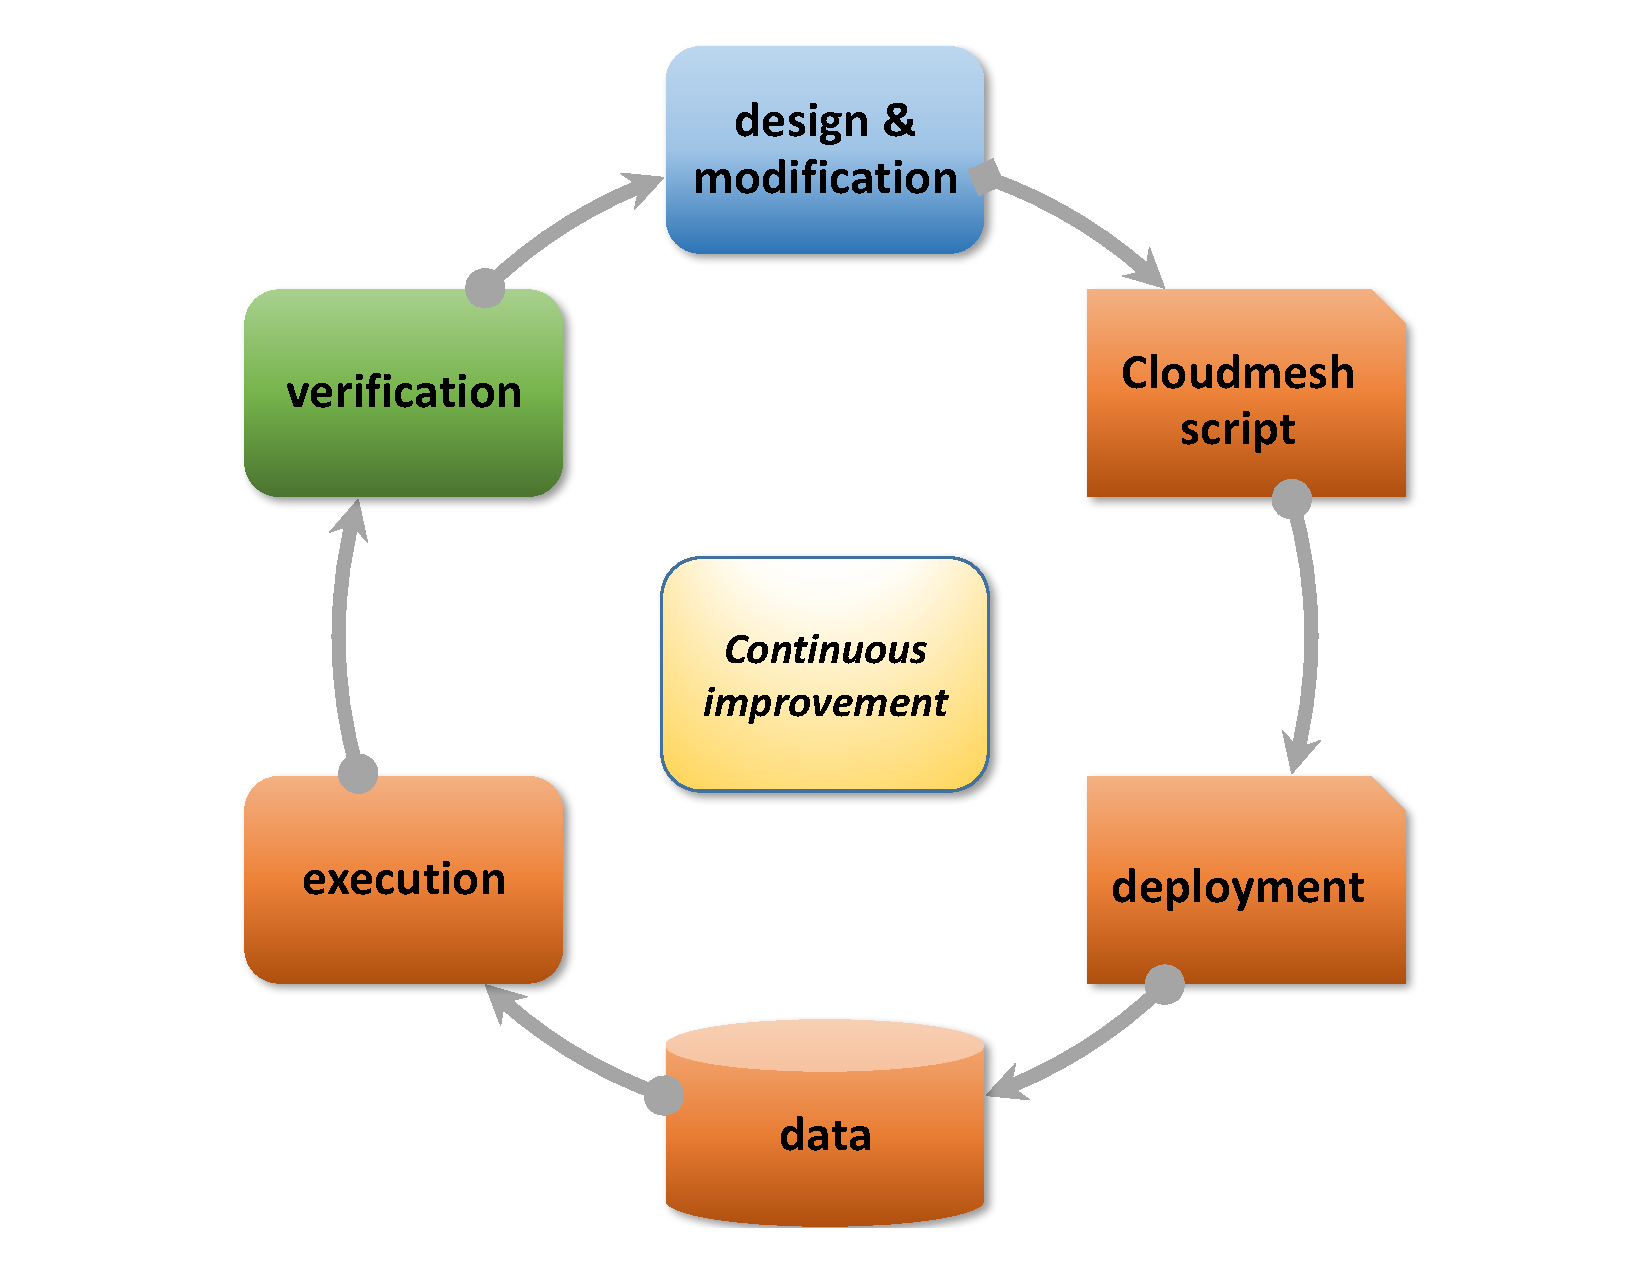
\includegraphics[width=1.0\columnwidth]{images/nist-devops-1.pdf}
  \caption{Continuous improvement while using cloudmesh interactively.}
  \label{F:NIST-devops-1}
\end{figure}


Figure \ref{F:NIST-devops-1} depicts a high level overview of the cyclic workflow
associated with a single application for a specific dataset. Starting
with a Cloudmesh Script that allocates resources and then deploys the
necessary software and desired dataset. The analytics component
executed is then executed. Upon verification of the results and
modification of compnenets as needed the process repeats. This
continues iteratively until the desired results are achieved. Tests at
the end that verify certain results will be used to verify if the
resulting run was successful. If not they are flagged and a
notification is send to the maintaining team. New big data tests can
be integrated into the set of benchmarks tested and the they can be
evaluated based continuously or upon change.


This behaviour is augmented in Figure~\ref{F:NIST-devops-2} with the integration of the
data repositories that are used to manage and maintain the scripts,
the playbooks and the data. While the scripts are simple cloudmesh
scripts to drive a particular application, we envision that most roles
are published as ansible roles to be integrated in application
specific playbooks. Playbooks exists for the phases of the execution

\begin{description}
\item[Phase 0:] start of the integrated application verification
\item[Phase 1:] setup of the infrastructure 
\item[Phase 2:] deployment of the platform and application
\item[Phase 3:] running a test on a specific data set.
\item[Phase 4:] verification of the result
\end{description}


\begin{figure}
  \centering
      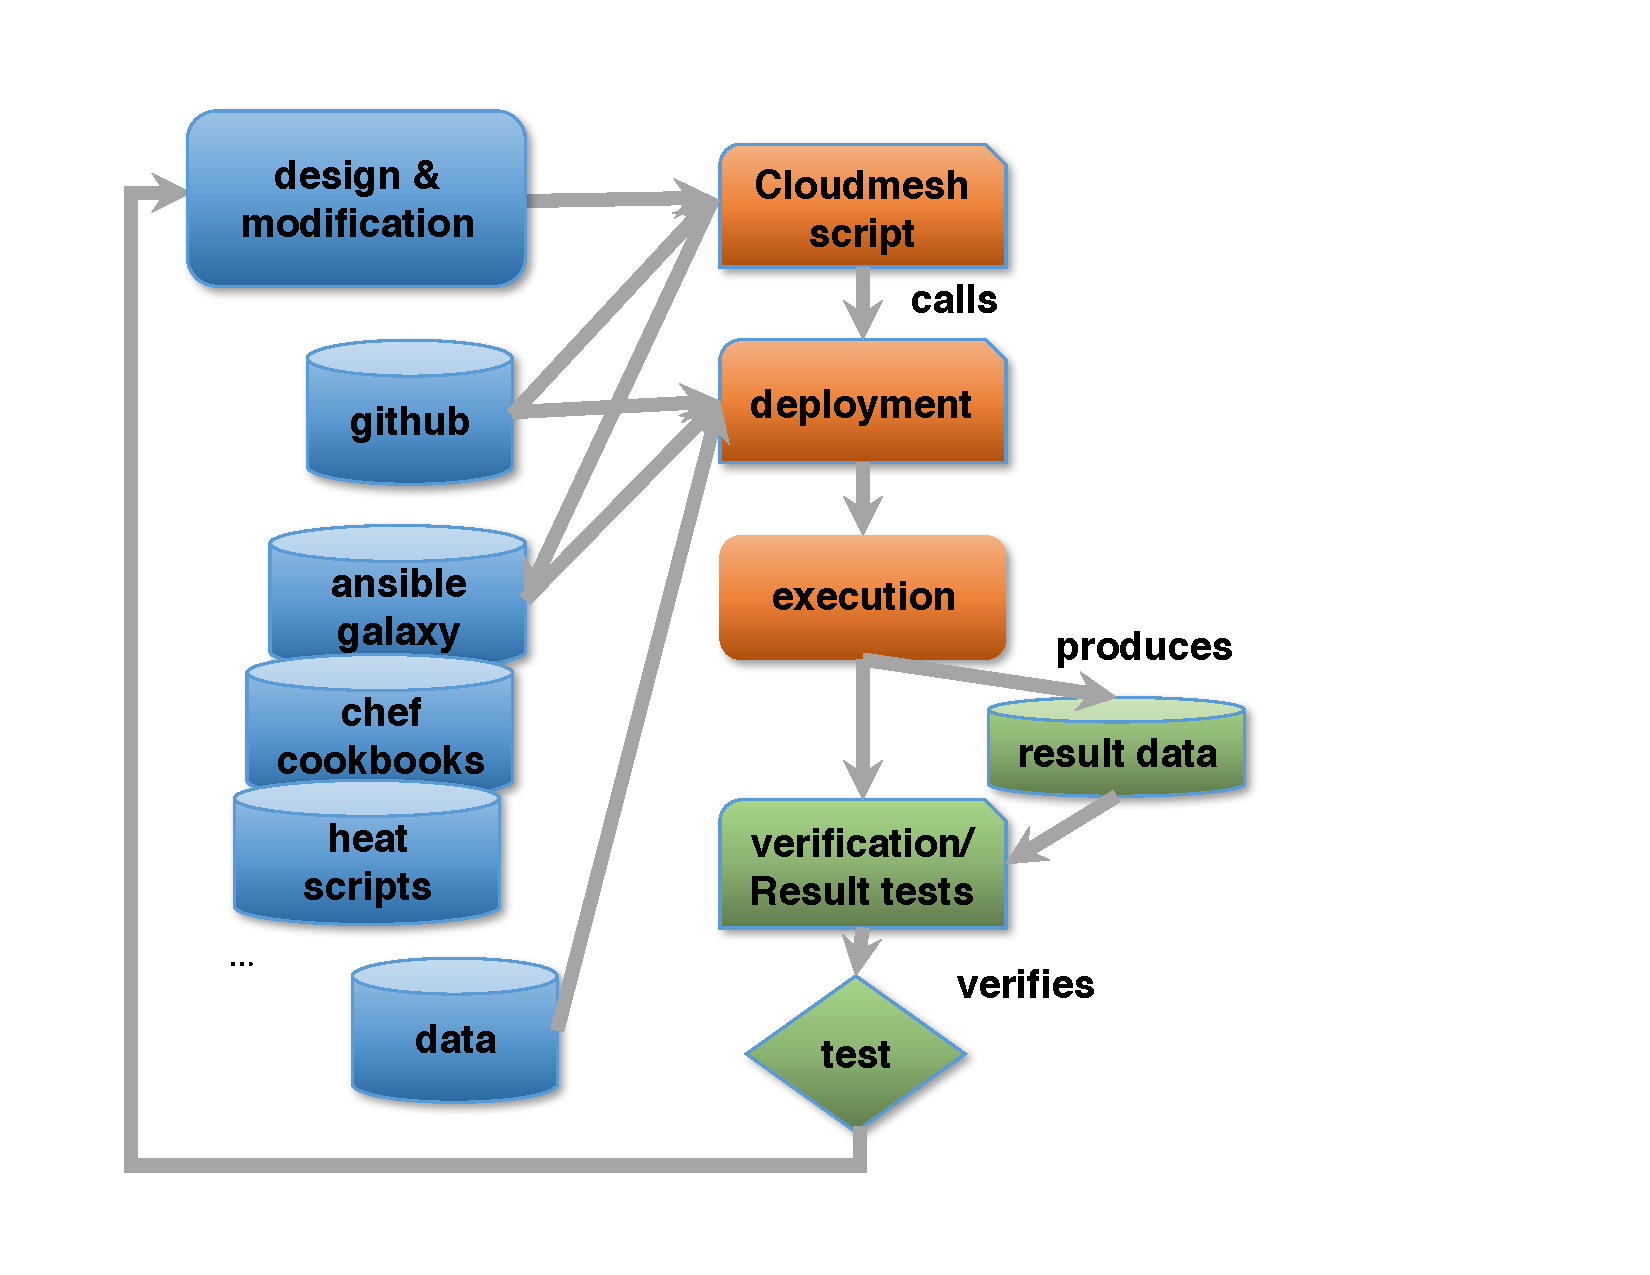
\includegraphics[width=0.8\columnwidth]{images/nist-devops-2.pdf}
  \caption{Interaction of the continuous improvement steps with
    various databases while using ansible deployment scripts.}
  \label{F:NIST-devops-2}
\end{figure}


\section{Software Stacks}

We will be describing multiple software components in later
sections. To put them into better context we provide a brief overview
here.

\begin{description}
\item[Support infrastructure.] Systems such as OpenStack, Amazon EC2,
  Amazon Azure, Google Compute Engine, Chameleon Cloud, Jetstream, San
  Diego Supercomputer Cluster's Comet. These are platforms that
  support allocating resources for computation, storage, and network. 
\item[DevOps.] Tools such as Ansible, Puppet, Chef, and others listed
  in Table~\ref{T:devops-tools} provide the ability to install
  software on and configure a virtual cluster allocated by the support
  infrastructure.
\item[Cloudmesh.] A client program which interfaces with multiple
  support infrastructure providers, allowing allocation of virtual
  clusters across multiple providers. This greatly aids the goal of
  scripting deployments. Additionally, pursuant of the same goal,
  Cloudmesh is beginning to use DevOps tools to configure the
  allocated resource.
\item[Big Data Stack.] A collection of curated Ansible playbooks for
  deploying common Big Data software such as Hadoop, Spark, or
  HBase. It is developed the Cloudmesh group and is used to support
  the DevOps portion of the Cloudmesh codebase.
\end{description}



\section{Provisioning Machines}



The first step in a data processing pipelines is the
provisioning/allocation of compute resources. These can be physical
machines or, increasingly common and accessible, virtual
machines. There are several major technologies that support this
infrustructure as a service paradigm. Some notable ones include Amazon
EC2, Microsoft Azure, Google Compute Engine, and Chameleon Cloud.


Part of our work has been in developing the cloudmesh client, which is
a lightweight client interface of accessing heterogeneous clouds,
clusters, and work- stations right from the users computer. The user
can man- age her own set of resources she would like to utilize. Thus
the user has the freedom to customize their cyber infras- tructure
they use. Cloudmesh client includes an API, a command-line client, and
a command-line shell. It strives to abstract backends to databases
that are used to manage the workflow utilizing the different
infrastructure and also the services. Switching for example to stage
virtual machines from OpenStack clouds to amazon is as simple as
specify- ing the name of the cloud. Moreover, cloudmesh client can be
installed on Linux, MacOSX, and in future Windows.  Currently
cloudmesh supports backends to SLURM, SSH, OpenStack, AWS, and
Azure. Using cloudmesh, users can migrate accross infrustructure
service providers relatively seemlessly.


\begin{figure}[htb]
  \centering
     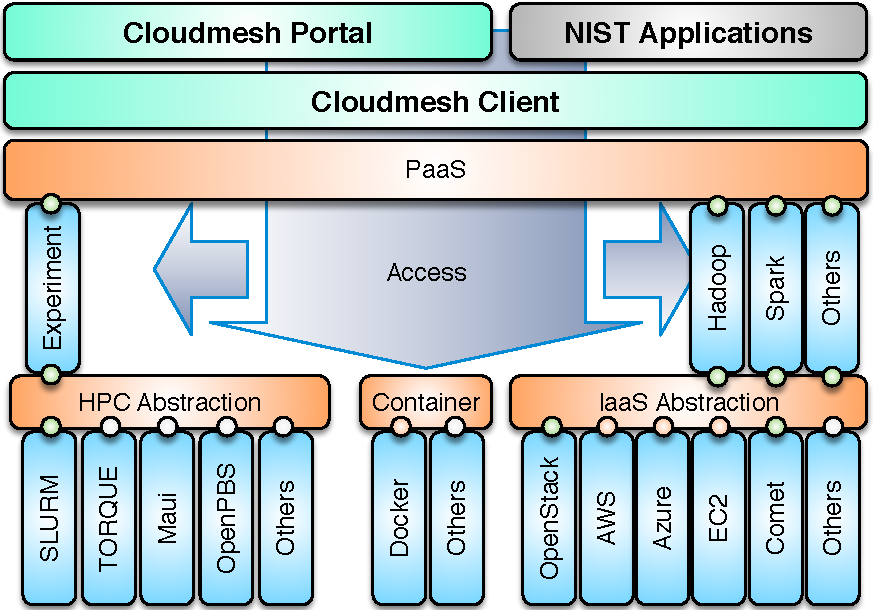
\includegraphics[width=1.0\columnwidth]{images/cloudmesh-arch-1.pdf}
  \caption{Cloudmesh layered architecture.} 
  \label{F:cloudmesh-arch}
\end{figure}


Figure~\ref{F:cloudmesh-arch} describes the architecture of Cloudmesh Client.

%\section{Deployment and Configuration of Software}
\section{Deployment and Configuration}

The second step of the pipelines consists of deploying the desired
software onto newly allocated resources. At this point, nodes may be
available, but are in their initial state, which needs to be updated
by installing and configuring software.


DevOps tools aim to support this component. One significant benefit is
the conceptualization of {/em code-as-infrastructure}, that is the
definitions of the desired state of the clusters are defined in text
files that can be checked into a version control system and tested.

\subsection{DevOps Tools}

The following table provides a short overview of several notable
DevOps tools. These tools allows the state of a cluster to be defined
at various levels. Some (such as Ansible, SaltStack) primarily operate
at the level of software deployment and configuration of a preexisting
cluster, while others (i.e. Juju, NixOps) additionally provide support
for allocating the compute resources. Another factor is the
interaction with the cluster via pushing the desired state to the
nodes, or having the nodes run an agent that pulls the state
definition and then evaluates it locally. Finally, the desired state
is either declaratively defined, where the tools determines the steps
required to achieve the state, or imperatively, where the
user/developer is responsible.


\begin{table*}[htb]
  \begin{center}
    \begin{small}
      \caption{List of notable DevOps tools.}
      \label{T:devops-tools}
      \begin{tabular}{|l|l|l|l|l|}

% https://www.ansible.com/
% https://www.chef.io/chef/
% https://puppet.com/
% https://cfengine.com/
% https://saltstack.com/
% https://pressly.github.io/sup/
% http://www.fabfile.org/
% http://inedo.com/otter
% https://jujucharms.com/
% https://nixos.org/nixops/


Tool         & Developer       & License          & Method    & Approach \tabularnewline \hline \hline
Ansible      & Ansible Inc.    & GPLv3            & Push      & Declarative            \tabularnewline \hline
Chef         & Chef            & Apache v2        & Pull      & Imperative             \tabularnewline \hline
Puppet       & Puppet          & GPL, Apache      & Pull      & Declarative            \tabularnewline \hline
CFEngine     & CFEngine AS     & GPLv3            & Pull      & Declarative            \tabularnewline \hline
SaltStack    & Thomas Hatch    & Apache v2        & Push+Pull & Declarative+Imperative \tabularnewline \hline
Sup          & Pressly, Inc    & MIT              & Push      & Imperative             \tabularnewline \hline
Fabric       & Jeffrey Forcier & Open Source      & Push      & Imperative             \tabularnewline \hline
Otter        & Inedo           & Proprietary      & Push      & Declarative+Imperative \tabularnewline \hline
Juju         & Canonical       & Affero GPL, LGPL & Push      & Declarative            \tabularnewline \hline
NixOps       & NixOS Community & GPLv3            & Push      & Declarative            \tabularnewline

      \end{tabular}
    \end{small}
  \end{center}
\end{table*}


Several of these tools may be used to showcase different capabilities:


\begin{description}

\item[Ansible] is a YAML-based declarative descriptions of the desired
  state of the system. The description is used to generate a Python
  program that is pushed over SSH to each node, where it is then run
  to modify the system.

\item[Chef] is a Ruby Domain Specific Language for defining sets of
  actions (or {/em recipes}). These recipes are pulled onto the
  managed nodes from a configuration server.

\item[Juju] focuses on connecting services together, using arbitrary
  tools to bring a system to the desired state.

\item[NixOps+NixOS] provide resource allocatoion (EC2, GCE, Azure) for
  NixOS nodes as well as DevOps deployment. Once started, the nodes
  are brought to the desired state by interpreting a configuration
  file which declaratively defines the desired state of the node.

\end{description}


\subsection{Concepts}

One of our design principles is to allow the user to use whichever
technologies they are most familiar with. Therefore we do not wish to
constrain them into using a specific DevOps technology such as Ansible
or Chef. Additionally, there are many deployment definitions for
various technologies publically available for these deployment
software, as well as private definitions housed by whichever company
developed them.


\begin{description}

\item[Cluster] A cluster is a collection of virtual machines that can
  be references as a group. Methods acting on the virtual cluster are
  restricted to adding and removing instances. This layer is
  responsible for allocating and deallocating resources (i.e. starting
  and stopping the instances).


\item[Stack.] A stack defines how a particular technology is to be
  deployed. This uses deployer plugins to support using Ansible Roles,
  Chef Recipes, NixOS configurations, etc. The core concept is that a
  Stack represents a single technology, such as Hadoop, or Spark, or
  HBase. One of the desired properties of Stack evaluation is
  idempotence. Evaluating a given Stack on a node multiple times
  should have the exact same effect on the state of the system as
  evaluating it once.


\item[Composition.] A Composition is a group of Stacks that as a whole
  represent the deployment of a group of technologies. For instance
  Figure~\ref{F:stack-composition} shows that in order to provide
  Fingerprint Matching as a service, one would need a Web stack, a
  Fingerprint stack, and the Hadoop stack.

  \begin{figure}
    \centering
    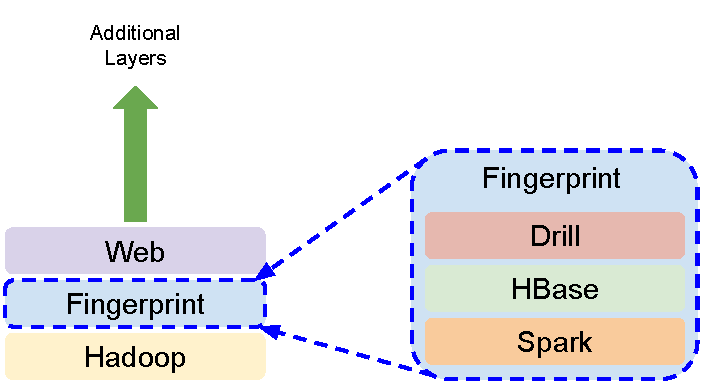
\includegraphics[width=1\columnwidth]{images/cloudmesh-stack-composition.pdf}
    \caption{Multiple stacks may be composed. Here, the
      {\it Fingerprint} stack is a composition of the Apache
      {\it Drill}, {\it HBase}, and {\it Spark}
      stacks. The {\it Fingerprint} stack is then included as a layer withing
      another composition built upon {\it Hadoop} and extended with the
      {\it Web} layers. The {\it Web} layer itself may be composed
      of other layers.
      \label{F:stack-composition}}
  \end{figure}

  Figure~\ref{F:stack-composition}. Fingprint Stack composed with Hadoop and Web stacks to
  provide Fingerprinting-as-a-Service. Note that Stacks can also be
  Compositions


  One crucial concept is that Stacks and Compositions are mutually
  recursive: a Composition is composed of at least one Stack, and each
  stack itself be a composition.


\item[Link.] A Link allowes services to introspect properties of the
  virtual cluster and other Stacks at the time of deployment. For
  example, during the deployment of Apache Hadoop, the Hadoop Stack
  needs to determine the address of the nodes running the Zookeeper
  service, as well as the port on which Zookeeper is
  exposed. Currently this information is maintained by hand, which
  causes deployments to be very sensistive to how dependent
  compositions are configured. The goal for Linking is to propagate
  this information throughout the Stack Composition dependency graph
  as needed.


\item[Deployment/Evaluation.] A Deployment defines DevOps
  application-specific interface to evaluate Compositions.
  Figure~\ref{F:stack-graph} shows how the sample Fingerprint service
  stack shown in Figure~\ref{F:stack-composition} may be
  evaluated. First the Daemon Watcher stack is deployed, as it is
  required by Hadoop. Although Java Stack is required for Hadoop,
  Spark, HBase, and Drill, it should only be evaluated once per
  node. The Fingerpring and Web stack may potentially be evaluated in
  parallel. The semantics of the parallel evaluation is not well
  understood at the moment though.


  
  \begin{figure}
    \centering
    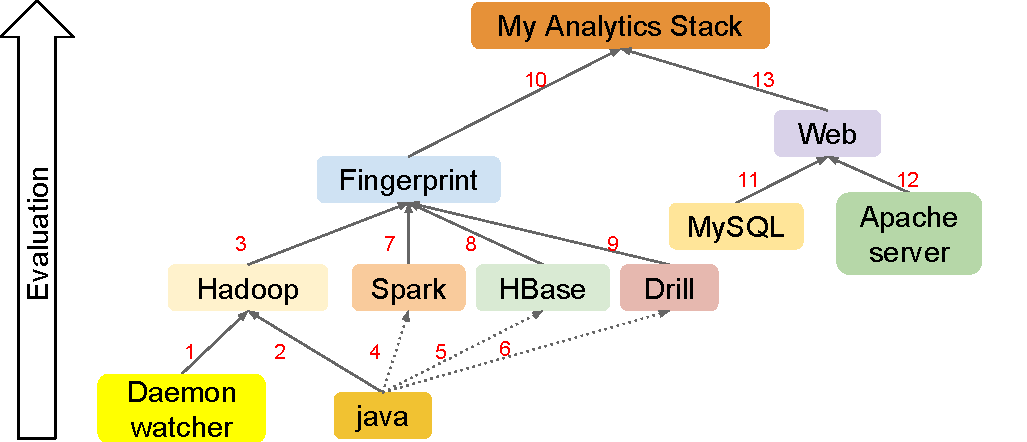
\includegraphics[width=1\columnwidth]{images/cloudmesh-stack-graph.pdf}
    \caption{Evaluation of a stack.
      The {\it My Analytics Stack} is composed of the {\it Fingerprint} and {\it Web} layers.
      These in turn are themselves compositions.
      Numbers indicate order of evaluation. While {\it spark}, {\it hbase}, and {\it drill} depend on {\it java}, re-evaluation (\textit{4} - \textit{6}) is not problematic due to the idempotency property.
      \label{F:stack-graph}}
  \end{figure}


  Figure~\ref{F:stack-graph}. Evaluation of a Stack shown as a dependency graph.


\end{description}


\subsection{Design Principles}

\begin{description}

\item[Client based.] As a client, the cloudmesh program requires no
  special privileges to run. This adheres to the principle of least
  priviledge in an attempt to minimize security issues. The program
  runs locally end exits completely once the user terminates it.


\item[Command Shell and Command Line Interface.] The enables scripting
  with cloudmesh as a way of automating virtual cluster deployment and
  tear down.


\item[Plugin Architecture.] The purpose of the plugins is to allow
  users to use the deployment tools they are most familiar with,
  without constraining them to a specific technology. Additionally, a
  desired outcome of this design is increased code sharing and reuse.


\item[REST API.] The goal here is that the client may be used to
  support service-based deployments, in scenarios that warrent it.


\item[Layered Architecture.] The layered architecture, as shown in
  Figure~\ref{F:cloudmesh-arch}, is intended to facilitate development
  and integration of different components that are not currently
  supported. For example, adding Docker support exposes a Docker layer
  that may be used to launch containers in a similar fashion to
  OpenStack virtual machines.


\item[Management Framework.] The supports management of allocated
  resources, allowing starting, stopping, restarting, reinitializing,
  etc.


\item[Database Agnostic.] The state of various components is stored in
  a database. Currently this is an SQLite database, but access to the
  database all passes through a dedicated module. The hope is that, if
  needed, the database backend may be parameterized to support others
  such as MariaDB, PostgreSQL, MongoDB, etc.

\end{description}


\subsection{REST API Development}

As described elsewhere, one of our goals is to provide a
Representational State Transfer (REST) API for cloudmesh. This would
enable web services to more easily use Cloudmesh to provide users with
the ability to use and manage virtual clusters.  REST is a well
understood and widely used approach for designing and developing
service-based APIs. Additionally the semantics of HTTP methods in a
REST context are defined.


Table~\ref{T:rest} shows an initial draft of the Cloudmesh REST
API. These show resources and how the HTTP methods may be used to
manage virtual clusters, stack compositions and deployments, and HPC
experiments.


\begin{table*}[htb]
  \bigskip
  \begin{center}
    \begin{small}
      \caption{Selected Service Description. Items prefixed with a colon (:) indicate parameters e.g. :id, :?.}
      \label{T:rest}
      \begin{tabular}{|l|l|l|}
        \hline
        \blue \textbf{Resource} & \blue \textbf{REST Method} & \blue \textbf{Description}\tabularnewline

%%%%%%%%%%%%%%%%%%%%%%%%%%%%%%%%%%%%%%%%%%%%%%%%%%%%%%%%%%%%%%%% Virtual cluster
\hline \multicolumn{3}{|l|}{\grey\bf Virtual Cluster: /cluster} \tabularnewline \hline
/                         & GET      & List available clusters \tabularnewline \hline
/                         & POST     & Launch a cluster on the provider \tabularnewline \hline
/                         & DELETE   & Delete all available clusters \tabularnewline \hline
/:id                      & DELETE   & Delete and destroy a cluster \tabularnewline \hline
/:id                      & GET      & View the status of a cluster (nodes, node type, etc) \tabularnewline \hline
/:id/properties/:property & GET, PUT & Get/set a property (provider, name, description) of the cluster \tabularnewline \hline
/:id/inventory/:format    & GET      & Obtain an inventory of the cluster \tabularnewline \hline

%%%%%%%%%%%%%%%%%%%%%%%%%%%%%%%%%%%%%%%%%%%%%%%%%%%%%%%%%%%%%%%% Composition
\hline \multicolumn{3}{|l|}{\grey\bf Stack Composition: /stack} \tabularnewline \hline
/                               & GET      & List available compositions \tabularnewline \hline
/                               & POST     & Create a new composition \tabularnewline \hline
/:id                            & GET      & Show information about the composition \tabularnewline \hline
/:id                            & DELETE   & Delete a composition \tabularnewline \hline
/:id/name                       & GET, PUT & Get/set the name of the composition \tabularnewline \hline
/:id/add?deployer=:?\&source=:? & POST     & Add a layer to the composition \tabularnewline \hline
/:id/layers                     & GET      & List layers of the composition \tabularnewline \hline
/:id/layers/:id                 & DELETE   & Delete the layer of the composition \tabularnewline \hline

%%%%%%%%%%%%%%%%%%%%%%%%%%%%%%%%%%%%%%%%%%%%%%%%%%%%%%%%%%%%%%%% Stack Deployment
\hline \multicolumn{3}{|l|}{\grey\bf Stack Deployment: /stack} \tabularnewline \hline
/                         & GET  & List the available stacks with discription \tabularnewline \hline
/:id/deployments/:cluster & POST & Deploy a stack onto a cluster \tabularnewline \hline
/:id/status               & GET  & Current status \tabularnewline \hline
/:id/deployments/:cluster & GET  & Current status on given cluster \tabularnewline \hline

 %%%%%%%%%%%%%%%%%%%%%%%%%%%%%%%%%%%%%%%%%%%%%%%%%%%%%%%%%%%%%%%% Batch
\hline \multicolumn{3}{|l|}{\grey\bf Batch Experiments: /hpc} \tabularnewline \hline
/                          & GET    & List all jobs started with the run command \tabularnewline \hline
/:id                       & DELETE & Deletes the experiment with the given id \tabularnewline \hline
/run?script=:?\&cluster=:? & POST   & Submits an experiment to the named cluster \tabularnewline \hline
/:id/status                & GET    & Returns the status of the job started with the run command \tabularnewline \hline

      \end{tabular}
    \end{small}
  \end{center}
\end{table*}

\section{Ecosystem Analysis}

We believe that big data ecosystem consists of various software,
applications and datasets on different platforms. To understand
current activities on big data projects and provide recommended
software components (roles) in big data, we conduct analysis on big
data projects 1) from community (i.e. github), 2) and academia
(i.e. indiana university) regarding to the following entities:

\begin{itemize}
\item development language preference
\item library/package/tool dependencies
\item sectors of public dataset source
\end{itemize}

This effort will result in building recommended software components
(roles) which supports most of functionalities in a given big data
applications.

\subsection{Analysis on Big Data Projects from Community}

Github.com has been used to provide version control and manage source
code development along with diverse collaborators across
countries. The popularity of github as a collaboration tool has been
significantly increased and 4,995,050 repositories exist as of
12/27/2016 with 20-30 thousands daily added repositories. To
understand trends on big data software development from community, we
conducted a survey of github repositories regarding to big data
applications and tools. Every github repository has a description of a
project and we searched them using topic keywords. For example, we
collected github repositories for Face Detection with search keywords;
face detection, face recognition, human detection, and person
detection to conduct a survey on a series of questions regarding to 1)
A development language distribution, 2) dependency of libraries and
packages, and 3) sectors of public dataset. Actual source code of
public github repositories are evaluated with the survey query data
available on
\url{https://github.com/lee212/bd_stats_from_github}. There are six
topics of NIST Collection used in this analysis where N1: Fingerprint
Matching, N2: Face Detection, N3: Twitter Analysis, N4: Data
Warehousing, N5: Geographic Information Systems, and N6: Healthcare
Data. In addition, a list of recommended components (roles) is created
based on the survey results.

\subsubsection{Language Preference}

The repository statistics indicate that C++, Python and Java are most common
languages among the NIST collection (Table~\ref{tab:language-distribution}),
although Matlab is dominant in the fingerprint.

\begin{table*}[htb]
  \begin{center}
    \begin{small}
      \caption{Language Distribution of Topics related to those in the NIST collection on Github}
      \label{tab:language-distribution}
      \begin{threeparttable}
	\begin{tabular}{l|l|l|l|l|l|l|l|l|l|l|l}

	  Topic & C++ &  Python &  Java &  Matlab &  JS &  C\# &  C &  R &  Ruby &  Scala &  Count\tnote{*} \tabularnewline \hline \hline
	  Fingerprint& 15\% & 11\% & 13\% & 20\% & 3\% & 16\% & 8\% & 0\% & 1\% & 5\% & 43 \tabularnewline \hline
	  Face & 26\% & 21\% & 12\% & 9\% & 7\% & 5\% & 2\% & 2\% & 1\% & .02\% & 538 \tabularnewline \hline
	  Twitter & 2\% & 35\% & 15\% & .6\% & 9\% & 2\% & 1\% & 10\% & 3\% & 1\% & 1429 \tabularnewline \hline
	  Warehousing & 3\% & 27\% & 18\% & 2\% & 10\% & 3\% & 1\% & 10\% & 4\% & 1\% & 3435  \tabularnewline \hline
	  Geographic & 5\% & 15\% & 27\% & 4\% & 15\% & 3\% & 5\% & 7\% & 3\% & 16\% & 6487 \tabularnewline \hline
	  Healthcare & 2\% & 13\% & 19\% & 2\% & 14\% & 5\% & 1\% & 10\% & 6\% & 2\% & 132 \tabularnewline

	\end{tabular}
	\begin{tablenotes}
	\item[*] Count: average number of github.com repositories.
	\end{tablenotes}
      \end{threeparttable}
    \end{small}
  \end{center}
\end{table*}

\begin{figure}[htb]
  \begin{center}
    \begin{small}
  \caption{Python Packages used in NIST Collection (collected from Github)}
  \centering
  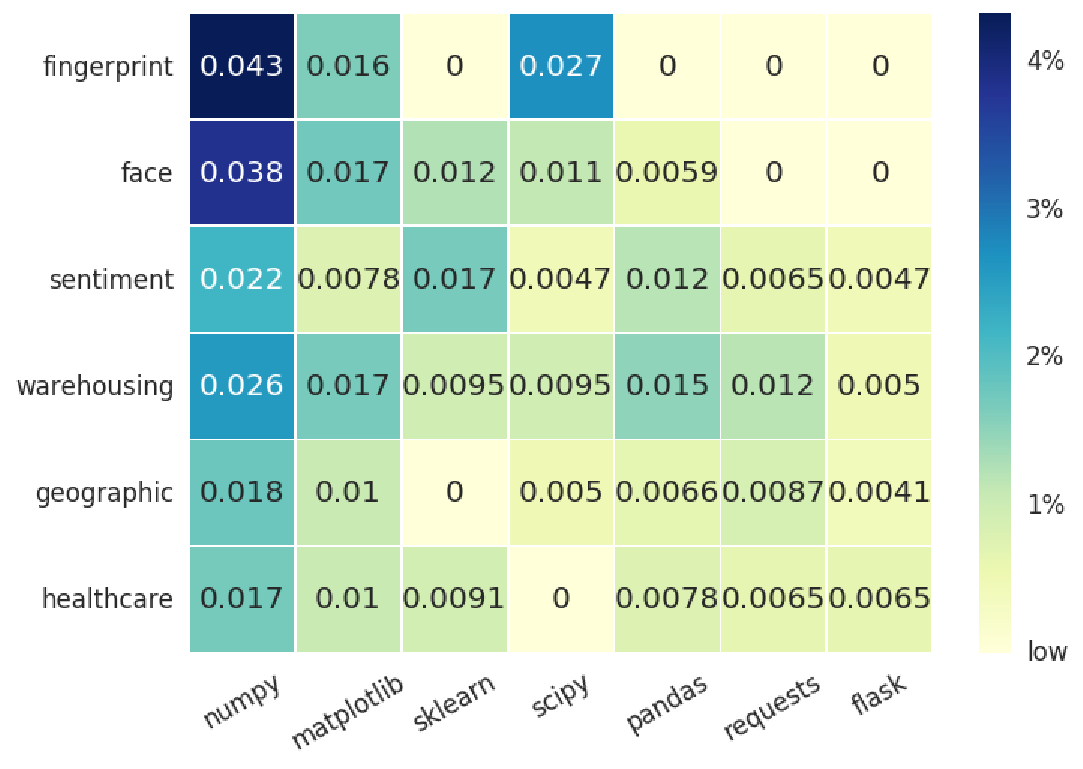
\includegraphics[width=0.5\textwidth]{images/packages-heatmap}
  \label{fig:packages-heatmap}
\end{small}
\end{center}
\end{figure}


\subsubsection{Package/Library/Tool Dependencies}

We also notice that scientific python packages are commonly used to enable
numerical computation, data analysis and visualization for these big data
applications (Figure~\ref{fig:packages-heatmap}), whereas there are dependent
packages for each project (Table~\ref{tab:additional-py-packages}). Tweepy,
twitter API, is used in the twitter live analysis projects with NLTK, the
natural language processing toolkit to complete sentiment analysis with
streaming data, tweets. Similarly, GIS projects use particular libraries for
spatial analysis such as geopy and shapely. New trends in software development
packages and libraries are observed, for example, deep learning python packages
e.g. caffe or theano have added recently to github repositories. Statistics
(tables\ref{tab:project-examples-face}) show that popular github repository
examples related to the six nist projects started in 2016. Each github project
has different language preferences with various libraries and packages however
similar trends are observed, for example, deep learning software such as Keras,
Theano, mxnet and Caffe are adopted among multiple projects.

\begin{table}[htb]
  \begin{center}
    \begin{small}
      \caption{Additional Python packages found in NIST Collection}
      \label{tab:additional-py-packages}
      \begin{tabular}{m{1.25cm}|m{2.25cm}|l|l|l|l|l|l}

    Python Package & Description              & \rot{Fingerprint} & \rot{Face} & \rot{Twitter} & \rot{Warehousing} & \rot{Geographic} & \rot{Healthcare} \\ \hline \hline
    cv2            & OpenCV                   & \OK               & \OK        &               &                   &                  &                  \\ \hline
    skimage        & Image Processing         &                   & \OK        &               &                   &                  &                  \\ \hline
    PIL            & Python Imaging           &                   & \OK        &               &                   &                  &                  \\ \hline
    caffe          & Deep Learning            &                   & \OK        &               &                   &                  &                  \\ \hline
    nltk           & Natural Language Toolkit &                   &            & \OK           &                   &                  &                  \\ \hline
    tweepy         & Twitter                  &                   &            & \OK           &                   &                  &                  \\ \hline
    Beautiful Soup & Screen scraping          &                   &            & \OK           & \OK               &                  &                  \\ \hline
    gensim         & Topic Modelling          &                   &            & \OK           & \OK               &                                     \\ \hline
    geopy          & Geocoding library        &                   &            &               &                   & \OK              &                  \\ \hline
    shapely        & Geometric Analysis       &                   &            &               &                   & \OK              &                  \\ \hline
    django         & Web framework            &                   &            &               & \OK               &                  & \OK              \\ 

      \end{tabular}
    \end{small}
  \end{center}
\end{table}


Additional packages (table~\ref{tab:additional-py-packages}) are not required
in a default set of big data ecosystem but it is necessary to indicate the
dependency with a particular application. 

\begin{table*}[htb]
  \begin{center}
    \begin{small}
      \caption{Example Projects Recently Created Regarding to Face Detection}
      \label{tab:project-examples-face}
      \begin{tabular}{p{2cm}|p{5cm}|l|l|l|p{3cm}}

    Title & Description & Language & Start Date & Popularity & Dependency \\ \hline  \hline
    OpenFace &  an open source facial behavior analysis toolkit & c++ & March, 2016 & 725 (305) & OpenCV, dlib, boost, TBB \\ \hline
    Picasso face detection transformation & An Android image transformation library providing cropping above Face Detection (Face Centering) for Picasso & Java & July, 2016 & 528(56) & Square Picasso \\ \hline
    MTCNN face detection alignment & Joint Face Detection and Alignment using Multi-task Cascaded Convolutional Neural Networks & Matlab & September, 2016 & 226(162)  &  Caffe, Pdollar toolbox \\ \hline
    facematch & Facebook Face Recognition wrapper & JavaScript & January, 2016 & 132 (41) & fbgraph, request, body-parser, express \\ \hline
    mxnet mtcnn face detection & MTCNN face detection & Python  & October, 2016 & 99 (47) & OpenCV, mxnet \\ 


  \end{tabular}
\end{small}
  \end{center}
\end{table*}


\subsubsection{Datasets}

Finding relevant datasets for particular applications is another challenge for
the big data ecosystem because of its difficulty of collecting data from
multiple sources (Kim, Trimi, and Chung, 2014), complexity and diversity
(Hashem et al., 2015). Community contributed lists of public datasets (Cohen
and Lo,2014) provide structured information with a specific location to access
data and a category to describe itself. We intend to generate linked json data
for datasets and applications in big data ecosystem based on these lists
because it connects scattered data and software in an organized way.
Table~\ref{tab:dataset-sector} shows the data source from different sectors,
academia(.edu or .ac), government(.gov), organization(.org), industry(.com or
.net), and international(country code in suffix), among the seven topics of the
lists. Entire topics are available online:
\url{https://github.com/lee212/bd_datasets}.

\begin{table}[htb]
  \begin{center}
    \begin{small}
      \caption{Public Dataset of acamedia, government, organization,
        industry and international from Community}
      \label{tab:dataset-sector}
      \begin{tabular}{l|l|l|l|l|l|l}

    Category         & \rot{Academia} & \rot{Government} & \rot{Organization} & \rot{Industry} & \rot{International} & Total \\ \hline \hline
    GIS              & 1              & 3                & 5                  & 9              & 5                   & 23    \\ \hline
    Healthcare       & 0              & 6                & 3                  & 1              & 1                   & 11    \\ \hline
    Image Processing & 11             & 0                & 4                  & 2              & 5                   & 18    \\ \hline
    Natural Language & 7              & 0                & 8                  & 7              & 6                   & 26    \\ \hline
    Social Networks  & 8              & 0                & 7                  & 5              & 5                   & 24    \\ \hline
    Climate/Weather  & 2              & 6                & 3                  & 2              & 4                   & 16    \\ \hline
    Energy           & 2              & 2                & 5                  & 1              & 5                   & 15    \\ 

      \end{tabular}
    \end{small}
  \end{center}
\end{table}


\subsection{Analysis on Big Data Projects from Academia}

At Indiana University, Big Data Analytics and Applications (BDAA) and
Big Data Open Source Software Projects (BDOSSP) have been offered in
2015 and 2016 accordingly. During these semesters, students have asked
to complete a course project with big data software, tools and
datasets. The choice of languages, software, and dataset are
surveyed in this section.

\subsubsection{Language Preference}

\begin{table}[htb]
  \begin{center}
    \begin{small}
      \caption{Language Distribution for Big Data Classes from Indiana University}
      \label{tab:lang-dist-iu}
      \begin{threeparttable}
        \begin{tabular}{l|l|l|l|l|l}

    Class      & Java & Python & R  & C\# & Projects Count \\ \hline \hline
    Fall '15   & 6    & 29     & 10 & 1   & 49             \\ \hline
    Spring '16 & 11   & 16     & 1  & 0   & 37             \\ \hline
    Fall '16   & 1    & 73     & 3  & 0   & 77             \\ 

        \end{tabular}
        % \begin{tablenotes}
        % \end{tablenotes}
      \end{threeparttable}
    \end{small}
  \end{center}
\end{table}



\subsubsection{Package/Library/Tool Dependencies}

We had 37 final projects from Big Data Open Source Project Spring 2016
and Table~\ref{tab:tools-sp16} shows that packages/tools/libraries used in the
class projects. Apache Hadoop is mostly used in conducting data analysis with a
database support from HBase, Hive and HDFS. Python was the most preferred
language in the course projects which resulted in high use of Spark in data
processing with the python library, pyspark. One another observation is that
Ansible, software deployment tool, had offered as a method of project
deployment to ensure reproducibility.

\begin{table}[htb]
  \begin{center}
    \begin{small}
      \caption{List of Top 15 Tools/Libraries/Packages used in Big
        Data Class Fall 2015}
      \label{tab:tools-fa15}
      \resizebox{\columnwidth}{!}{
        \begin{tabular}{l|l|l|l|l}

    Package      & Type      & Use                       & Language        & Count\tnote{*} \\ \hline \hline
    Numpy        & library   & data management           & Python          & 13             \\ \hline
    Pandas       & library   & data management           & Python          & 10             \\ \hline
    Matplotlib   & library   & visualization             & Python          & 8              \\ \hline
    Scipy        & library   & data management           & Python          & 6              \\ \hline
    Mongodb      & database  & NoSQL                     & C++             & 10             \\ \hline
    Hadoop       & framework & parallel processing       & Java            & 6              \\ \hline
    Nltk         & library   & NLP                       & Python          & 5              \\ \hline
    ggplot2      & library   & visulization              & R               & 4              \\ \hline
    scikit-learn & library   & machine learning          & Python          & 7              \\ \hline
    IPython      & Tool      & Web Interface \& Notebook & Python          & 4              \\ \hline
    Tableau      & Tool      & visualization             & C++             & 4              \\ \hline
    rstudio      & Tool      & development IDE           & R               & 3              \\ \hline
    seaborn      & library   & visualization             & Python          & 3              \\ \hline
    Spark        & framework & in-memory processing      & Scala           & 3              \\ \hline
    Randomforest & library   & classification            & R               & 2              \\ \hline
    Hbase        & database  & NoSQL                     & Java            & 2              \\ \hline
    Folium       & library   & visualization             & Python          & 2              \\ \hline
    MPI          & framework & parallel processing       & C, C++, Fortran & 2              \\ \hline
    Pig          & language  & data processing           & Java            & 2              \\ 

        \end{tabular}}
        \begin{tablenotes}
        \item[*] Count: a number of class projects in a given tool/library/package
        \end{tablenotes}
    \end{small}
  \end{center}
\end{table}

\begin{table}[htb]
  \begin{center}
    \begin{small}
      \caption{List of Top 15 Tools/Libraries/Packages used in Big Data Class Spring 2016}
      \label{tab:tools-sp16}
      \begin{threeparttable}
 \resizebox{\columnwidth}{!}{
  \begin{tabular}{l|l|l|l|l}

    Package   & Type      & Use                           & Language   & Count\tnote{*} \\ \hline \hline
    Hadoop    & framework & parallel processing           & Java       & 31             \\ \hline
    Ansible   & tool      & deployment                    & Python     & 26             \\ \hline
    Spark     & framework & in-memory processing          & Scala      & 14             \\ \hline
    HBase     & database  & NoSQL                         & Java       & 12             \\ \hline
    Pig       & language  & data abstraction              & Java       & 11             \\ \hline
    Hive      & database  & SQL                           & Java       & 7              \\ \hline
    MongoDB   & database  & NoSQL                         & C++        & 7              \\ \hline
    Mahout    & library   & machine learning, data mining & Java       & 4              \\ \hline
    MLLib     & library   & machine learning              & Java       & 4              \\ \hline
    OpenCV    & library   & computer vision               & C++        & 3              \\ \hline
    Zookeeper & framework & directory service             & Java       & 3              \\ \hline
    Tableau   & tool      & visualization                 & C++        & 3              \\ \hline
    D3.js     & tool      & visualization                 & Javascript & 2              \\ \hline
    MySQL     & database  & SQL                           & C++        & 2              \\ \hline
    HDFS      & database  & distributed filesystem        & Java       & 2              \\ 

  \end{tabular}}
  \begin{tablenotes}
  \item[*] Count: a number of class projects in a given tool/library/package
  \end{tablenotes}
  \end{threeparttable}
    \end{small}
  \end{center}
\end{table}

\begin{table}[htb]
  \begin{center}
    \begin{small}
      \caption{List of Top 15 Tools/Libraries/Packages used in Big
        Data Class Fall 2016}
      \label{tab:tools-fa16}
      \begin{threeparttable}
        \resizebox{\columnwidth}{!}{
        \begin{tabular}{l|l|l|l|l}

    Package      & Type     & Use                    & Language & Count\tnote{*} \\ \hline \hline
    Matplotlib   & library  & visualization          & python   & 88             \\ \hline
    Pandas       & library  & data management        & python   & 79             \\ \hline
    Numpy        & library  & data management        & python   & 65             \\ \hline
    Scipy        & library  & data management        & python   & 24             \\ \hline
    Requests     & library  & http tool              & Python   & 22             \\ \hline
    xlrd         & library  & MS Excel               & Python   & 10             \\ \hline
    pillow       & library  & imaging library        & Python   & 9              \\ \hline
    scikit-learn & library  & machine learning       & Python   & 9              \\ \hline
    seaborn      & library  & visualization          & Python   & 8              \\ \hline
    nltk         & library  & language processing    & Python   & 6              \\ \hline
    geopy        & library  & geospatial tool        & Python   & 5              \\ \hline
    pyOpenSSL    & library  & OpenSSL                & Python   & 5              \\ \hline
    patsy        & library  & statistics             & Python   & 5              \\ \hline
    bokeh        & library  & visualization          & Python   & 4              \\ \hline
    ploty        & library  & visualization          & Python   & 4              \\ \hline

        \end{tabular}}
        \begin{tablenotes}
        \item[*] Count: a number of class projects in a given tool/library/package
        \end{tablenotes}
      \end{threeparttable}
    \end{small}
  \end{center}
\end{table}


\subsubsection{Datasets}

There were 49 class project in Big Data Analytics and applications Fall 2015,
and use of 27 dataset are observed. Public dataset from industry was mainly
used (44\%) due to the interest on analytics from kaggle and twitter and
availability e.g. amazon reviews and yelp reviews.

\begin{table}[htb]
  \begin{center}
    \begin{small}
      \caption{Dataset Sectors of academia, government, organization,
        industry and international from Big Data Classes at Indiana
        University}
      \label{tab:dataset-sector-iu}
      \begin{tabular}{l|l|l|l|l|l|l}

    Class & \rot{Academia} & \rot{Government} & \rot{Organization} & \rot{Industry} & \rot{International} & Total \\ \hline \hline
    Fall '15   & 7          & 3            & 5       & 12        & 0             & 27    \\ \hline
    Spring '16 & 6          & 6            & 8       & 10         & 1             & 30    \\ \hline
      \end{tabular}
    \end{small}
  \end{center}
\end{table}



\section{Selected Applications}

\subsection{Fingerprint Matching}

Implementation repository\\
\url{https://github.com/cloudmesh/example-project-nist-fingerprint-matching}

\subsubsection{Description}

Fingerprint recognition refers to the automated method for verifying a
match between two fingerprints and that is used to identify
individuals and verify their identity. Fingerprints
(Figure~\ref{F:NIST-fingerprints}) are the most widely used form of
biometric used to identify individuals.



\begin{figure}[htb]
  \centering
      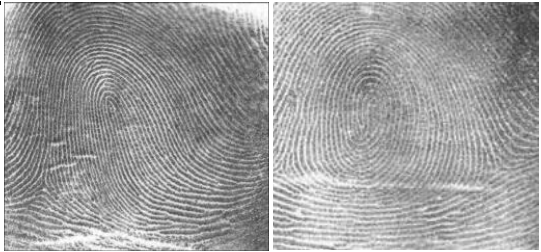
\includegraphics[width=0.9\columnwidth]{images/fingerprints}
  \caption{Example Fingerprints.}
  \label{F:NIST-fingerprints}
\end{figure}



The automated fingerprint matching generally required the detection of
different fingerprint features (aggregate characteristics of ridges,
and minutia points) and then the use of fingerprint matching
algorithm, which can do both one-to- one and one-to- many matching
operations. Based on the number of matches a proximity score (distance
or similarity) can be calculated.


The goal for this project is: given a set of probe and gallery images,
compare the probe images to the gallery images, and report the
matching scores.  The dataset used comprises 54,000 images along with
their metadata. Provided tools include MINDTCT and BOZORTH3, which are
part of the NIST Biometric Image Software (NBIS) release. These two
tools form the core of the application: MINDTCT preprocesses the
images to identify minutae which is used by BOZORTH3 to compute a
match.


The implemented solution uses stack of HDFS, YARN, Apache Spark,
Apache HBase, and Apache drill. A Hadoop cluster is deployed and YARN
used to schedule Spark jobs that load the images into HBase, process
the images, and compute the matches. Apache Drill, with the HBase
plugin, can then be used to generate reports.

\subsubsection{Software Stack}

\begin{itemize}
\item Big Data software packages:

\begin{itemize}
\item Apache Hadoop (YARN)
\item Apache Spark
\item Apache HBase
\item Apache Drill
\end{itemize}

\item Datasets:
\begin{itemize}
\item NIST Special Database 14 - Mated Fingerprint Card Pairs 2.
\end{itemize}

\item Domain Specific code (NBIS):
\begin{itemize}
\item MINDTCT
\item BOZORTH3
\end{itemize}


\item Other tools and technologies:
\begin{itemize}
\item Scala
\end{itemize}

\end{itemize}

\subsubsection{Deployment Approach}

The resource allocation can be done using Cloudmesh Client.
Next, Cloudmesh Big Data Stack is used to deploy the Big Data software packages.
Finally, some Ansible playbooks deploy and compile a scala program that integrates the Big Data infrustructure with running the domain specific code.

\subsubsection{Development Status}

Complete

% \subsubsection{Lessons Learned}

\subsection{Face Detection}

Implementation repository:\\
 \url{https://github.com/futuresystems/pedestrian-and-face-detection}

\subsubsection{Description}

Human detection and face detection have been studied during the last
several years and models for them have improved along with Histograms
of Oriented Gradients (HOG) for Human Detection~\cite{dalal2005histograms}.
OpenCV is a Computer Vision library including the SVM classifier and the HOG
object detector for pedestrian detection and INRIA Person Dataset
~\cite{dalal2005inria} is one of popular samples for both training and testing
purposes. This example shows how to deploy the NIST Human and Face Detection
with INRIA Person Dataset to the cluster where we deployed Apache Spark on
Mesos to train and apply detection models from OpenCV using Python API. OpenCV
Python code runs with Spark Map function to perform distributed job processing
on the Mesos scheduler.

\begin{figure}[htb]
  \centering
      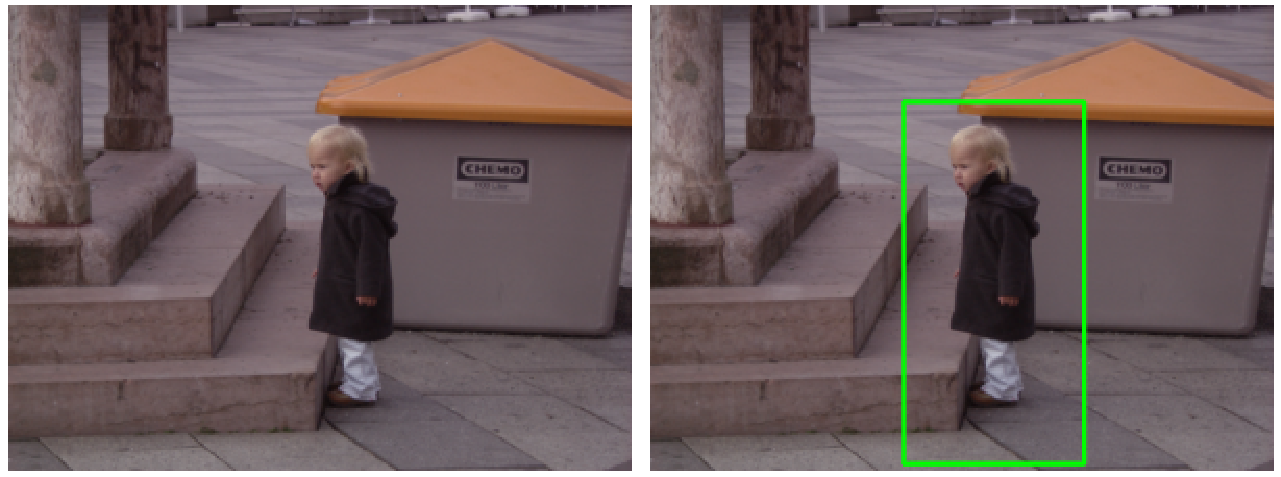
\includegraphics[width=0.9\columnwidth]{images/human_detection}
      \caption{Human Detection, original image (left), processed image (right)}
  \label{F:NIST-face1}
\end{figure}

\begin{figure}[htb]
  \centering
      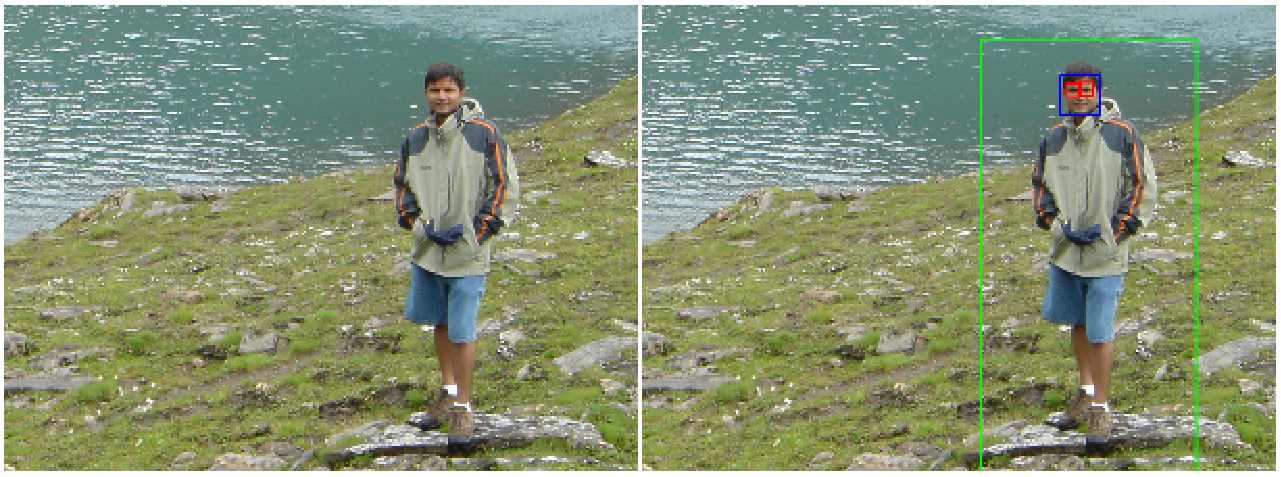
\includegraphics[width=0.9\columnwidth]{images/face_eye_detection}
    \caption{Face and Eye Recognition with Human Detection (face: blue box, eye: red box, human: green box)}
  \label{F:NIST-face2}
\end{figure}

\subsubsection{Software Stack}

\begin{itemize}

\item Big Data software packages:

\begin{itemize}
\item Apache Spark
\item Apache Mesos
\item Apache Zookeeper
\item OpenCV (with Python)
\end{itemize}

\item{Datasets:}


\begin{itemize}
\item INRIA Person Dataset
\end{itemize}

\end{itemize}

\subsubsection{Deployment Approach}

Mesos role is installed with two Ansible inventory groups; masters and
slaves where mesos-master runs on the masters group and mesos-slave
runs on the slaves group. Apache Zookeeper is included in the mesos
role and mesos slaves find an elected mesos leader from the
zookeeper. Spark, as a data processing layer, provides two options for
distributed job processing, batch job processing via a cluster mode
and real-time processing via a client mode. The Mesos dispatcher runs
on a masters group to accept a batch job submission and Spark
interactive shell, which is the client mode, provides real-time
processing on any node in the cluster. Either way, Spark is installed
after a scheduler layer i.e. mesos to identify a master host for a job
submission. Installation of OpenCV, INRIA Person Dataset and Human and
Face Detection Python applications are followed.

\subsubsection{Development Status}

Complete

% \subsubsection{Lessons Learned}


\subsection{Twitter Analysis}

\subsubsection{Description}

Social messages generated by Twitter have been used with various
applications such as opinion mining, sentiment analysis (Pak and
Paroubek, 2010), stock market prediction (Bollen, Mao, and Zeng,
2011), and public opinion polling (Cody et al., 2016) with the support
of natual language toolkits e.g. nltk (Bird, 2006), coreNLP (Manning
et al., 2014) and deep learning systems (Kim, 2014). Services for
streaming data processing are important in this category. Apache Storm
is widely used with the example of twitter sentiment analysis, and
Twitter Heron, Google Millwheel, LindkedIn Samza, and Facebook Puma,
Swift, and Stylus are available as well~\cite{chen2016realtime}.

\subsubsection{Software Stack}

Big Data software stack:

\begin{itemize}
\item Apache Hadoop
\item Apache Lucene
\item Twitter Heron
\item Apache Storm
\item Apache Flume
\item Natural Language Toolkit (Python)
\item gensim NLP library
\end{itemize}



\subsection{Analytics for Healthcare Data and Informatics}

\subsubsection{Description}

Several attempts have been made to apply Big Data framework and
analytics in health care with various use cases. Medical image
processing, signal analytics and genome wide analysis are addressed to
provide efficient diagnostic tools and reduce healthcare costs (Belle
et al., 2015) with big data software such as Hadoop, GPUs, and
MongoDB. Open source big data ecosystem in healthcare is
introduced~\cite{raghupathi2014big} with examples and challenges to satisfy big
data characteristics; volume, velocity, and
variety~\cite{zikopoulos2011understanding}. Cloud computing framework in
healthcare for security is also discussed with concerns about
privacy~\cite{stantchev2014cloud}.


\subsubsection{Software Stack}

Big Data software stack:

\begin{itemize}
\item Apache Hadoop
\item Apache Spark/mllib
\item Apache Mahout
\item Apache Lucene/Solr
\item Theano deep learning library
\end{itemize}



\subsection{Spatial Big Data/Statistics/Geographic Information Systems}

\subsubsection{Description}

The broad use of geographic information system (GIS) has been increased over
commercial and scientific communities with the support of computing resources
and data storages. For example, Hadoop-GIS~cite{aji2013hadoop}, a high
performance spatial data warehousing system with Apache Hive and Hadoop, offers
spatial query processing in parallel with MapReduce, and
HadoopViz~\cite{eldawy2016hadoopviz}, a MapReduce framework for
visualizing big spatial data, supports various visualization types of data from
satellite data to countries borders.


\subsubsection{Software Stack}

\begin{itemize}
\item Apache Hadoop
\item Apache Spark/mllib
\item GIS-tools
\item Apache Mahout
\item GDAL - Geospatial Data Abstraction Library
\item S2 Geometry Library
\item geopy geocoding python library
\end{itemize}




\subsection{Data Warehousing and Mining}

\subsubsection{Description}

Researches in data warehousing, data mining and OLAP have investigated
current challenges and future directions over big data software and
applications~\cite{cuzzocrea2013data} due to the rapid
increase of data size and complexity of data models. Apache Hive, a
warehousing solution over a hadoop~\cite{thusoo2009hive}, has introduced to
deal with large volume of data processing with the other research
studies~\cite{chen2010cheetah,he2011rcfile} and NoSQL
platforms~\cite{chevalier2015implementing} have discussed with data warehouse
ETL pipeline~\cite{goodhope2012building}.


\subsubsection{Software Stack}

Big Data software stack:

\begin{itemize}
\item Apache Hadoop
\item Apache Spark/mllib
\item MongoDB
\item Hive
\item Pig
\item Apache Mahout
\item Apache Lucene/Solr
\item MLlib
\item Google BigQuery
\end{itemize}

\section{Application Status}

\subsection{Deployment Approach}

The resource allocation can be done using Cloudmesh Client.  Next,
Cloudmesh Big Data Stack is used to deploy the Big Data software
packages.  Finally, some Ansible playbooks deploy and compile
additional packages that integrates the Big Data infrastructure with
running the domain specific code.

\subsection{Development Status}


Fingerprint Matching
Facetetection
twiter analysis
analytics for healthrcre data and informaticst
spacial big data / statistics / geographic information systems
data warehousing and mining

\FIXME{Planned}




\section{Components (Roles)}

Based on the analysis from community and academia, we observed that
there are crucial software, dataset and analytics in big data
ecosystem. We, therefore, offer deployable first-class roles which
enable major functionalities on big data processing and analysis. The
software deployment is accommodated with Cloudmesh, Ansible, Chef,
Puppet, Salt, OpenStack Heat, Microsoft Azure Template, and Amazon
Cloudformation.

\begin{itemize}
\item Framework
\begin{itemize}
   \item Hadoop
   \item Mesos
\end{itemize}
\item Processing
\begin{itemize}
   \item Spark
   \item Storm
\end{itemize}
\item Language
\begin{itemize}
   \item Pig
   \item R
\end{itemize}
\item Database
\begin{itemize}
   \item HBase
   \item Hive
   \item MongoDB
   \item MySQL
\end{itemize}
\item Library
\begin{itemize}
   \item Mahout
   \item nltk
   \item MLlib
   \item Lucene/Solr
   \item OpenCV
\end{itemize}
\item Tools
\begin{itemize}
   \item Ganglia
   \item Nagios
   \item Zookeeper
\end{itemize}
\end{itemize}


In detail, table is provided:

\begin{table*}[htb]
  \begin{center}
    \begin{small}
      \caption{Dataset Sectors of academia, government, organization,
        industry and international from Big Data Classes at Indiana
        University}
      \label{tab:dataset-sector-iu}
      \begin{tabular}{l|m{3cm}|l|m{2cm}|m{2cm}|m{2cm}|m{2cm}}

	Role Name & Description & Type & Requirement (Installation) & Dependencies & Distributed & Example \tabularnewline \hline \hline
	Spark & In-memory data processing application & processing & JDK 7+ Maven 3.3.9 & Hadoop (optional) & 	Cluster Manager/Executor (Worker node) & 	  \\ \hline
	hadoop & Map/Reduce distributed processing framework & framework & JDK & Resource Manager/Node Manager & & WordCount   \\ \hline
	Storm &	a real time fault-tolerant and distributed stream data processing system & processing & OpenJDK & ZooKeeper & Master/Worker &	\\ \hline
	Zookeeper & Synchronization service for distributed processes & tool & JDK 6+ &  & Ensemble (3 servers minimum) & 	\\ \hline
	hbase &	NoSQL database for real-time processing & database & JDK & ZooKeeper & Master / RegionServer & \\ \hline
	Twitter REST APIs & Reading Twitter data & library & 	 & OAuth & &  \\ \hline
	D3, tableau &  Javascript visualization library & visualization & &  & &  \\ \hline
	Nltk & Natural Language Toolkit & library & Python2.7 or 3.2+ & Numpy (optional) & 	 & \\ \hline
	AlchemyAPI & Collecting Tweets & library & Mongodb, R (ggplot2) & 	 &  & \\ \hline
	OpenCV & Computer Vision Libraries & library &  & &  &  \\ \hline
	Mahout & Machine learning applications & library & JDK Maven & hadoop-client & Via Hadoop, Spark, H20 or Flink & Naive Bayes (Classification) K-Means (Clustering) Recommender \\ \hline
	Lucene/Solr & Search engine framework & library & JRE 1.8+ & 	 & SolrCloud & 	 \\ \hline
	MLlib & Machine Learning Library from Spark & library & & Spark & & Logistic regression (Classification) K-means (Clustering) \\ \hline
	MongoDB & Document-oriented database & application & & & mongos/shard & \\ \hline
	Hive & Database SQL query interface to apache hadoop & application & JDK  Hadoop & 	Hadoop &  &  \\ \hline
	Pig & High level scripting language for Hadoop & Application & 	Hadoop JDK Ant (optional) JUnit (optional) &  & & \\ \hline
	RethinkDB & NoSQL, distributed document-oriented (JSON) database & application &  & & sharding, replication & \\ \hline
	TextBlob & Natural language processing (NLP) Python library & 	Analytics & 	NLTK corpora & & & \\ \hline
	Pattern & Web mining python library & 	Analytics & 	Numpy (for LSA; Latent semantic analysis) & 	Python 2.5+ only, no support on 3 &  & \\ \hline

      \end{tabular}
    \end{small}
  \end{center}
\end{table*}



\section*{Acknowledgements}

This work was in part supported by the NIST project {\it NIST-70NANB15H247}.

% Bibliography

\bibliography{references}
 



\end{document}
